\newpage
\section{Bartosz Toś}


\[e^i*e^\pi + 1 = 0\]


epicka akrtyczna małpa \ref{fig:maupa}
\begin{figure}[htbp]

    \centering
    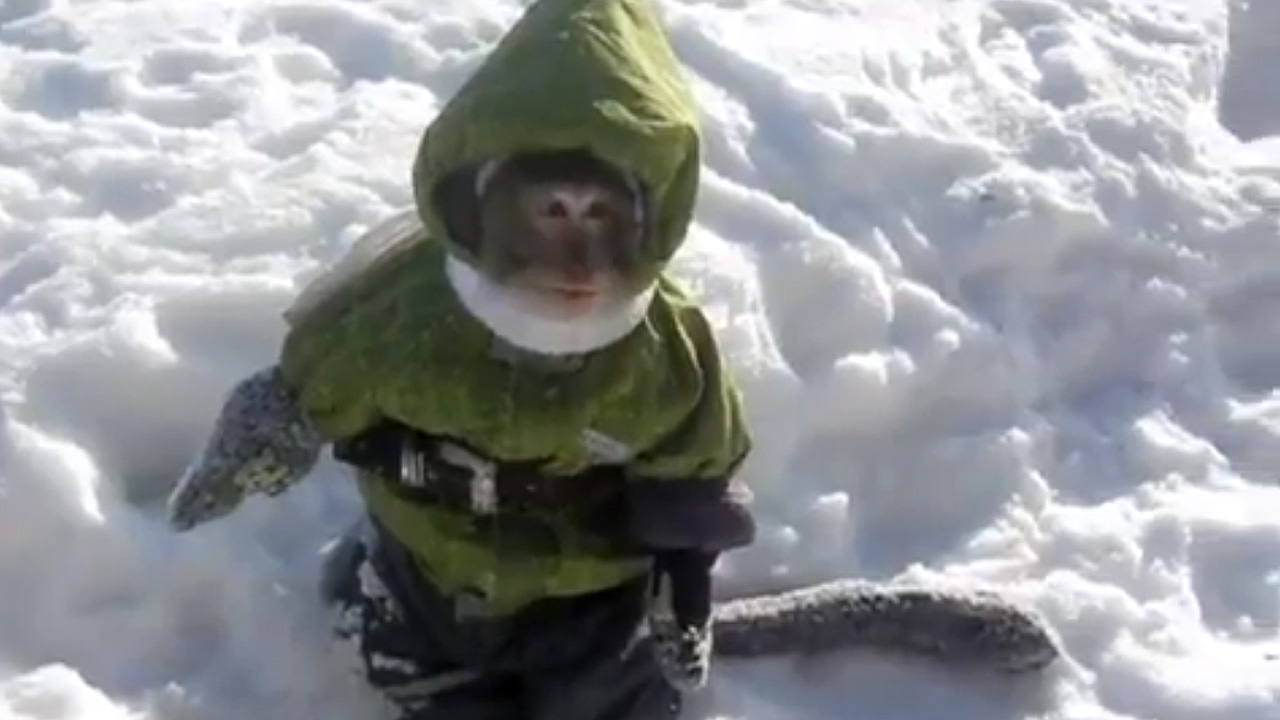
\includegraphics[scale=0.25]{pictures/arktyczna_maupa.jpg}
    
    \caption{maupa}
    \label{fig:maupa}
\end{figure}

\vspace{9 cm}

\textbf{tabela \ref{tab:matematyczne}:}
\begin{table}[]
\centering
\begin{tabular}{|c|c|}
\hline
\textbf{algebra} & \textbf{analiza} \\ \hline
miodzio          & świetna          \\ \hline
super            & ekscytujaca      \\ \hline
mega             & wspaniała        \\ \hline
genialna         & cudowna          \\ \hline
\end{tabular}
\label{tab:matematyczne}
\caption{przemyślenia na temat przedmiotów matematycznych}
\end{table}

\vspace{2 cm}

lista nienumerowana:

\begin{itemize}
  \item  1
  \item  2
  \item  3
\end{itemize}

\begin{itemize}
  \item[)]  1
  \item[)]  2
  \item[)]  3
\end{itemize}


lista numerowana:
\begin{enumerate}
  \item  1
  \item  2
  \item  3
\end{enumerate}
\vspace{2 cm}
\par
\begin{flushleft}
I've seen things you people wouldn't believe.
Attack ships on fire off the shoulder of Orion.
I watched c-beams glitter in the dark near the Tannhäuser Gate 
\emph{All those moments will be lost in time, like tears in rain.}
\end{flushleft}
\begin{flushright}
\par
\underline{Time to die.} 
\end{flushright}